Arrays are nice, simple ways to store blocks of data,
but we do not always know the necessary array size right off the bat.
How many spaces should we reserve/allocate? 
Allocating up to an arbitrary size (say, 1000) is not a good idea,
because it may be too much or too little memory for particular cases.

Dynamically sized arrays, which we saw in
Chapter~\ref{chap:dynamic-memory},
provide a partial solution to the problem:
at least, we do not need to know the array size at \emph{compile time}.
But we do still need to know how large to make the array at \emph{run time}
when we declare it. 
How large do you think that Facebook should have made its user array
when it started?
If you have more and more customers arriving over time,
it will be very hard to guess the ``right'' size.\footnote{%
  Of course, we could allocate some array dynamically,
  and when it gets too small, we allocate a larger array and copy over
  all the data. In fact, we will analyze this exact data structure in
  Chapter~\ref{chap:arraylists}.
  But the linked lists covered in this chapter serve to explain many
  important fundamental concepts you will need later.}

We will be looking at many data structures that do not
need to know the required number of elements beforehand;
rather, their size can dynamically change over time. 
Perhaps the easiest such data structure is called the
\todef{linked list};
it nicely illustrates many of the techniques we will see reappear many
times later. 

Consider how an array (dynamically or statically allocated) stores
data. Whenever new users arrive, a really convenient way of dealing
with it would be to just ask the operating system to expand our block
of memory to the required size.
However, there is no way to do this, and with good reason:
the memory right after our array may be in use for some other data,
so expanding our array may overwrite existing memory just after our
array's memory block. 
A way to ``expand'' our array may be instead to just get a second
block of memory somewhere else, and put a pointer at the end of our
first block to indicate where the next chunk is. 
This loses many of the advantages of arrays,
such as being able to do simple arithmetic to look up elements.
But at least, it would solve the problem in principle.

Once we think about growing an array that way,
we could go to the extreme and make \emph{every} element of our
``array'' point to the next element, removing all semblance of an array. 
This is what a linked list is: a series of nodes where each node points
to the next one in memory, and each node contains a piece of data.
We often depict linked lists as in Figure~\ref{fig:linkedlist}:

\begin{figure}[htb]
\begin{center}
\setlength{\unitlength}{1cm}
\begin{picture}(6,3)
\linethickness{0.1mm}
\multiput(0,0)(3,0){3}{%
\put(0,1.5){\framebox(2,1.5){value}}
\put(0,0){\framebox(2,1.5){next $\bullet$}}
}

\put(1.5,0.75){\vector(3,1){1.5}}
\put(4.5,0.75){\vector(3,1){1.5}}
\put(7.5,0.75){\vector(3,1){1.5}}
\put(-2,0){\vector(2,1){2}}
\put(10,0){\vector(-3,1){2}}
\put(-3,0){\code{head}}
\put(10,0){\code{tail}}
\end{picture}

\caption{Basic illustration of a linked list \label{fig:linkedlist}}
\end{center}
\end{figure}

Linked lists can be made as long as you want without declaring an
initial size first.
All you have to do is attach a node after the last one,
and ensure that the previously last element of the list now
points to the new last element.

Some analogies to keep in mind for linked lists are the following:
\begin{itemize}
\item A treasure hunt for children. The parents provide a clue for the
  first treasure. When the children figure out the clue, they go
  there, and find a treasure, along with a note that has the next clue.
  Following that clue, they get to the second treasure, where they find
  another note with a clue to the next treasure, and so on.
  The clues play the role of pointers.
\item The game of ``Assassin,'' in which each participant gets the
  name of another participant to ``kill'' in an agreed-upon way
  (shooting with a nerf gun, touching with a plastic spoon, etc.).
  When one participant is ``killed,'' his killer inherits his next
  assignment, and the winner is the last survivor.
  Again, the assignments can be thought of to form a linked list
  (except the tail points back at the head).
\item There are several other analogies of sequential structures,
  like dominoes, train cars, and others.
  What's nice about the two examples above is the explicit nature of
  the ``pointers.''
\end{itemize}

Many students will at this point be familiar with the C++
\code{vector} data type,
and remember that it has a \code{push\_{}back} function,
which seems to do something very similar to appending a new item at
the end of a linked list.
So what is the difference between a \code{vector} and a linked list,
and why do we have to learn about linked lists when vectors are so
convenient?

Vectors are in fact covered in detail in
Chapter~\ref{chap:arraylists}, and we will compare them in more detail
there.
Roughly speaking, vectors act like arrays,
which means that you can access elements by position,
whereas linked lists do not give you direct position-based access.
In return, linked lists are perhaps a bit more efficient to implement.
More importantly, though, they are the simplest and cleanest
illustration of how to build data structures with many different
pieces pointing to each other,
and such data structures will be central later in this class.
Understanding how data structures such as vectors are built is one of
the main goals of this, and practicing on easier examples like linked
lists will get you ready for the more complicated structures later on.

\section{Implementing Linked Lists}
Each node/element in the linked lists contains data
(such as an \code{int}, \code{string}, etc.)
as well as a pointer to the next node/element of the same type. 
Here, we will build a linked list of integers
--- it should be pretty obvious how to alter it for other data.
In order to keep track of the data and the pointer,
we create a \code{struct} which we call \code{Node}. 

\begin{verbatim}
struct Node {
        int value;
        Node *next;

        Node (int val, Node *n)
        { value = val; next = n; }
}
\end{verbatim}

Every \code{Node} has an \code{int}
--- a piece of data in the linked list ---
and a pointer \code{next} to another node. 
The first node will have a pointer to the second node,
the second to the third, and so on. 
For the last node, we need a way to make sure to remember that there is
no more node after it.
The most common way is to have its \code{next} pointer point to \code{nullptr},
but some people instead have the last node's \code{next} pointer point
to itself.\footnote{When implemented correctly, there is really not a
  major advantage to either approach.
  A slight advantage of \code{nullptr} might be that your code will
  crash instead of running into an infinite loop when you do not check
  correctly for the end of the list --- crashes are typically easier
  to diagnose and pin down than infinite loops.}

The function \code{Node} we declare inside the \code{struct} is used
to make initialization easy.
This way, we can just write \code{Node* p = new Node (5, nullptr); }
instead of
\code{Node *p = new Node; p->value = 5; p->next = nullptr}.
It is called a \todef{constructor} of the \code{class} or \code{struct},
and you will learn about constructors in Chapter~\ref{chap:classes}.

The \code{struct Node} we defined helps us store the contents of any
one node.
In order to actually access the linked list, we also need a pointer to
the first element of the list.
From the first element, we can find the second element, then the third,
etc., by following the \code{next} pointers.
The pointer to the first element of the list is called the \code{head}
pointer.
If we ever lose track of it (for instance, by overwriting the variable
it was stored in),
we will not be able to access any part of the linked list any more,
and all of its memory will be leaked.
If you think back to the example of the treasure hunt for children,
none of the treasures will be found if the parents do not provide the
description of where to find the first treasure.
All the hints stored with the treasures will be useless then.

\subsection{Linked list operations}
In order for the list to be useful, at a minimum,
we want to be able to add elements to our list,
remove them, and traverse the entire list.
Here is how to implement those operations.

\begin{description}
\item[Traversal:] Unlike arrays, linked lists do not supply
  functionality to directly access the \Kth{i} element.
  Instead, we start from the first node (the head) and then visit the
  next node repeatedly. 
  To do so, we declare a variable 
  \code{Node *p}
  that will keep track of the current node we are looking at.
  \code{p} starts out as the pointer to the \code{head} element. 
  Then in each iteration of a \code{for} loop, we update it to its
  next pointer. So the code looks like this:
\begin{verbatim}
void traverse (Node *head)
{
   for (Node *p = head; p != nullptr; p = p->next)
     { // Do something with p, such as print or modify its data
     }
}
\end{verbatim}

  We can also traverse a list recursively, as follows:
\begin{verbatim}
void traverse (Node *p)
{
  if (p != nullptr) {
    // Do something with head, such as print or modify its data
    traverse (head->next);
  }
}
\end{verbatim}

The nice thing about the recursive implementation (besides its extreme
simplicity) is that it is very easy to make it traverse the list in
\emph{reverse} order, even if the list is singly linked.
You simply change the order of the two statements, calling
\code{traverse (head->next)} \emph{before} doing the processing
(such as the printing).
The task of printing a linked list in reverse order is a
very popular job/internship interview question,
because it tests knowledge of both linked lists and recursion.

\item[Addition:]
  To add a piece of data to an existing linked list,
  we take our input data item and create a new \code{Node} from it.
  This new node will typically be appended to the end of the list,
  so its \code{next} pointer will be set to \code{nullptr}. 
  (We could also add it at the beginning of the list, which would change
  the implementation below.)
  In order to append it at the end of the list, we first need to find
  the last element (called the \code{tail} of the linked list),
  then set its \code{next} pointer to the new node. 

  We need a special case when the list starts out empty,
  for in that case, we also have to set the \code{head} pointer which
  was previously \code{nullptr}.
In summary, the code for adding a new element looks as follows:
\begin{verbatim}
void append (Node *&head, int n)
{
  Node *newElement = new Node (n, nullptr);
  if (head == nullptr) head = newElement;
  else { 
        Node *p = head;
        while (p->next != nullptr) p = p->next;
        p->next = newElement;
       }
}
\end{verbatim}

Notice the somewhat strange-looking construction of the
\code{Node *\&{}head}.
We want to pass the head of the list, which is a \code{Node *}.
But we may also need to change it (in the case when it started out as
\code{nullptr}), so we need to pass the pointer by reference.

A somewhat shorter implementation can be obtained by using recursion:
\begin{verbatim}
void append (Node *&head, int n)
{
  if (head == nullptr) head = new Node (n, nullptr);
  else append (head->next, n);
}
\end{verbatim}

Notice that both the recursive and the iterative implementation have
to traverse the entire list to find the last element.
This is rather inefficient, and unnecessarily so.
This is why typically,
it is a good idea to not only maintain a \code{head} pointer,
but also a \code{tail} pointer to the last element of the list.
That way, we do not have to traverse the entire list every time we
want to add something.

\item[Removal:] 
If we are given a pointer \code{Node *toRemove} to an
element of the list that we would like to remove,
we will eventually deallocate its memory with
the command \code{delete toRemove}. 
But before that, we also need to make sure that the link structure of
the list stays intact.
To do so, we need a pointer \code{prev} to the element right before
\code{toRemove} in the list,
so that we may set \code{prev->next = toRemove->next;} 

One way to get this pointer (if it exists --- otherwise,
\code{toRemove} itself must be the \code{head} of the list) is to
start from the beginning of the list and scan through until we find
the node \code{p} with \code{p->next == toRemove}. 
That works fine, but would take a long time and be cumbersome.

The better solution is to store in each \code{Node} not only
a pointer to the next element in the list,
but also to the previous element.
The result is called a \todef{doubly linked list}, and unless
you have a strong reason to prefer a singly linked list
(such as a job interview or homework assignment specifying it), 
you would normally make your linked list doubly linked. 
In the definition of \code{Node}, we add the line \code{Node *prev}.
In the function for adding an element, we set 
\code{newElement->prev = nullptr} in the first case,
and \code{newElement->prev = p} in the second case.

\begin{figure}[htb]
\centering
\includegraphics[scale=0.6]{comics/xkcd_forgetting.eps}
\caption{XKCD \# 379: Forgetting}
\end{figure}

For removing an element, we can now write:
\begin{verbatim}
void remove (Node *&head, Node *toRemove)
{
  toRemove->prev->next = toRemove->next;
  toRemove->next->prev = toRemove->prev;
  delete toRemove;
}
\end{verbatim}
This sets the \code{next} pointer of the preceding element to the
\code{next} pointer of the element to be deleted, effectively
unlinking it. 
Similarly, the second line sets the \code{prev} pointer of the next
element to the \code{prev} pointer of the element to be deleted. 
While this looks good at first sight,
we have to be more careful when the element we want to remove is the
head or tail of the list
(or both, if the list happened to consist of a single element).
Then, \code{toRemove->prev} or \code{toRemove->next} could be \code{nullptr},
which means we cannot change their pointers.
Instead, we will need to update the head or tail of the list:

\begin{verbatim}
void remove (Node *&head, Node *toRemove)
{
  if (toRemove != head) 
     toRemove->prev->next = toRemove->next;
  else head = toRemove->next;
  if (toRemove->next != nullptr) 
     toRemove->next->prev = toRemove->prev;
  delete toRemove;
}
\end{verbatim}
\end{description}

The real reason for having doubly linked lists is that they
make deletions much easier and cleaner.
A side benefit is that a doubly linked list can be easily traversed
back to front.
Some textbooks list this as a reason for having a doubly linked list,
but we think that that it is a red herring:
first, traversing a linked list back to front is not hard even for a
singly-linked list if you use recursion.
And second, it is not a functionality that is often needed.

Once you really wrap our head around the idea of having the
\code{Node} class contain a pointer (or two) to other \code{Node} elements,
you may ask why not have more pointers to more \code{Node} elements. 
In fact, that is exactly what you will be learning about when we get
to more complex data structures such as trees later on.

\section{Recursive Definition of Linked Lists}

We now know intuitively what a linked list is, and we know how to
implement one. But we have not defined it formally.
In other words, we have not yet said exactly how to distinguish 
``A Linked List'' from a ``Not A Linked List.''
In trying to come up with a definition,
our intuition tells us that it is a bunch of items,
where each item has associated data and points to another item.
But first of all, one of the items does not point to anything.
And second, this would include a lot of nodes,
all of which point to \emph{the same} other node.
That is not what we want.
We may try something like ``a bunch of items, each of which points to
one other node, and is pointed to by one other node,
except for one node that points to no other node and one node which is
not pointer to by any other. And they all point to different nodes.''
This would perhaps be correct, but it is getting a little cumbersome.

To keep the definition short yet clear,
we can draw on recursive definitions which we introduced in
Section~\ref{sec:recursion:definitions}.
A recursive definition of Linked Lists looks as follows:

\begin{itemize}
\item The empty list is a linked list.
\item If $L$ is a linked list, then you obtain another linked list by
  taking a new node $v$ and having its next pointer point to $L$.
\end{itemize}

This definition captures exactly all linked lists,
and nothing that is not a linked list.
For example, it rules out a node pointing to itself.

In the implementation of linked lists we saw before,
the empty list was represented by \code{head==nullptr},
while non-empty lists had \code{head!=nullptr}.